\documentclass[../main/main.tex]{subfiles}

\begin{document}

\section{April  4th, 2019}
\subsection{Fractional Min-cut}
\textbf{Review} - LP relaxation of integer LP for min cut\\

\begin{tabular}{rl}
	minimize: &$\sum_{(u,v)\in e}c(u,v)y(u,v)$\\
	subject to: & $\sum_{(u,v)\in p}y(u,v) \ge 1,\quad\forall p\in p$\\
				&$y(u,v)\ge 0,\quad\forall (u,v)\in e$
\end{tabular}\\
$y(u,v)$ can be thought of the length of an edge, with the constraints being that the length of  $t$ from $s$ is at least 1.\\

To prove that the integrality gap to be 1, we need to show that there exists a integer cut that is just as good as the fractional min-cut

\begin{lemma}
	Given any feasible solution $y(u,v)$ for $(u,v)\in E$, it is possible to find a $s-t$ cut $A$ such that \[
		c(A) \le  \sum c(u,v)y(u,v)
	.\] 
\end{lemma}
Constraints of LP imply $d(t)\ge 1$. \\

Pick $T$ (threshold) uniformly at random in interval $[0,1)$. Define $A$ to be the set $A=\{v\ :d(v) \le T\}$, if $1$ was included in the interval, then $t$ could be in $A$. Now, we will show that \[
	E[c(A)]\le \sum c(u,v)y(u,v)
.\] If this is true, then we have proven the above lemma, as there cannot be a cut $A$ which has less capacity then the fractional min-cut. As it's less than or equal to the fractional min-cut, then they must be equal. For this to be consistent, then all edges crossing $A$ are 1, and everything else is $0$.\\
\begin{figure}[h!]
	\centering
	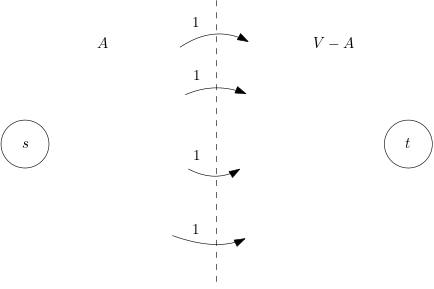
\includegraphics[width=0.6\textwidth]{4-4-frac-min-cut-t}
	%\caption{4-4-frac-min-cut-t}
	\label{fig:4-4-frac-min-cut-t}
\end{figure}
There must be a $s-t$ cut $A$ s.t. this is true, (since it is true on average).
\begin{proof}
	Define a random variable $X(u,v)$ to be 1 if $u\in A$ and $v\not\in A$. Otherwise it is $0$. \\
	\[
		c(A)=\sum_{(u,v)\in E} X(u,v)c(u,v)
	\] \[
	E[c(A)]=E[\sum X(u,v)c(u,v)
	.\] By the linearity of expectation:
	\[
		=\sum c(u,v)E[X(u,v)],\]
		\[ \quad E[X(u,v)] = \text{Pr}[X(u,v)=1]=\text{Pr}[d(u)\le T \text{ and }d(v)>T]\le d(v)-d(u)
	\] 
	\begin{figure}[h!]
		\centering
		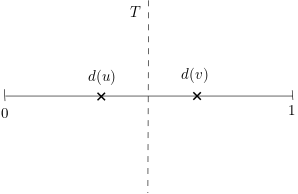
\includegraphics[width=0.6\textwidth]{4-4-du-dv}
		%\caption{}
		\label{fig:}
	\end{figure}\[
	d(v)\le d(u)+y(u,v)
	\]
	\[
		E[X(u,v)]\le d(v)-d(u)\le y(u,v)
	.\]  
\end{proof}
\subsection{Steiner Forest Problem}\index{Steiner forest}
Given a graph $G=(V,E)$, edge cost $C:E\to R^{+}$. In the Steiner tree problem, we have a set of required vertices that must be connected. In the Steiner Forest problem, we have sets $S_i \subseteq V$, find a minimum cost subgraph $F$ (for forest) such that each pair of vertices belonging to the same set $S_i$ is connected.\\

\textbf{Problem Restatement} Define a connectivity requirement function $r$ (for requirement) that maps unordered pairs of vertices to $\{0,1\}$: \[
	r(u,v) = \begin{cases}
		1,\quad \text{if $u$ and $$ belong to some set $S_i$}\\
		0,\quad \text{otherwise}
\end{cases}
\] Note that there cannot be cycles (can remove an edge to reduce the cost)\\
\begin{figure}[h!]
	\centering
	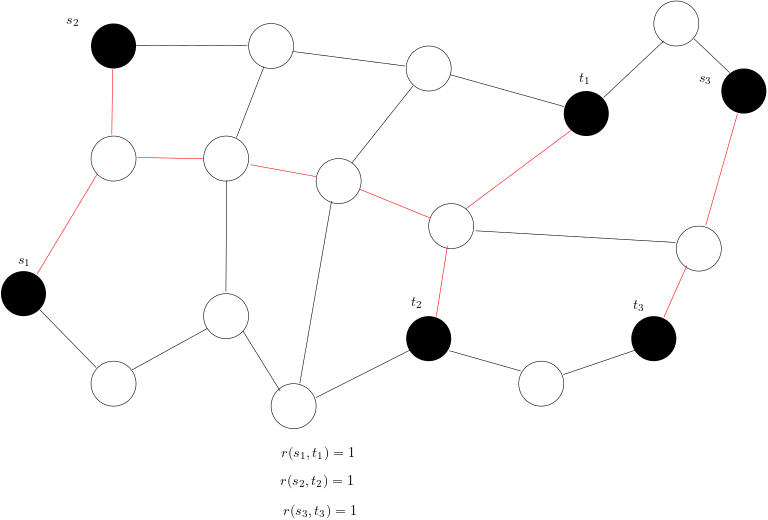
\includegraphics[width=\textwidth]{4-4-example-sf}
	\label{fig:4-4-example-sf}
\end{figure}
The ILP is: 
\begin{tabular}{rl}
	minimize: &$\sum_{e\in E} c_e x_e$\\
	subject to: & \ldots\\
				&$x_e \in \{0,1\} $
\end{tabular} but what are the constraints

Note that if $r(u,v)=1$, for every $u-v$ cut, there must be an edge crossing such cut. This is a necessary condition, but is it sufficient? It is, as if $u$,  $v$ were not connected, there would have been a cut that separates them.\\

We let  $\delta(S)$ denote the set of edges with exactly one endpoint in $S$. Let $\overline{S}=V-S$. Consider any cut $(S,\overline{S})$ in $G$ that separates a pair $(u,v)$ that should be connected. Then we \textbf{must} pick at least one edge $e\in \delta(S)$. Clearly this is necessary, but it is also sufficient.\\

Let $S^{\star}$ be the collection of all sets $S$ such that $(S,\overline{S})$ separate a pair $(u,v)$ for which $r(u,v)=1$. Introduce a 0/1 variable  $x_e$ for each edge $e\in E$:\\

Integer LP for Steiner Forest:\\

\begin{tabular}{rl}
	minimize: &$\sum_{e\in E} c_e x_e$\\
	subject to: & $\sum_{e:e\in \delta(S)}x_e\ge 1\quad \forall S\in S^{\star}$\\
				&$x_e \in \{0,1\} $
\end{tabular}\\

This is because each $S\in S^{\star}$ is a cut that must be crossed.
\end{document}
